\documentclass[11pt]{article}
% Shared preamble for report.tex and summary.tex (pdflatex, single column, US letter).
\usepackage[T1]{fontenc}
\usepackage[utf8]{inputenc}
\usepackage{lmodern}
\usepackage[letterpaper, margin=1in]{geometry}
\usepackage[final]{microtype}
\usepackage{amsmath, amssymb}
\usepackage{textcomp}
\usepackage{newunicodechar}
\newunicodechar{η}{\ensuremath{\eta}}
\newunicodechar{±}{\ensuremath{\pm}}
\newunicodechar{×}{\ensuremath{\times}}
\newunicodechar{→}{\ensuremath{\rightarrow}}
\newunicodechar{·}{\textperiodcentered}
\newunicodechar{⁷}{\textsuperscript{7}}
\newunicodechar{⁸}{\textsuperscript{8}}
\usepackage{graphicx}
\usepackage{xcolor}
\definecolor{fkgblue}{HTML}{2F6FBF}
\usepackage{booktabs, array, tabularx, xltabular, makecell}
\renewcommand{\arraystretch}{1.18}
\setlength{\tabcolsep}{5pt}
\usepackage{enumitem}
\setlist{itemsep=2pt, topsep=4pt, leftmargin=1.4em}
\usepackage[font=small, labelfont=bf, margin=0pt]{caption}
\usepackage{float}
\usepackage{tikz}
\usetikzlibrary{arrows.meta, positioning, fit, backgrounds, calc}
\usepackage{listings}
\lstdefinestyle{base}{basicstyle=\ttfamily\footnotesize, columns=fullflexible, keepspaces=true, breaklines=true,
  breakatwhitespace=false, frame=single, rulecolor=\color{black!25},
  framesep=4pt, xleftmargin=4pt, xrightmargin=4pt, aboveskip=6pt, belowskip=6pt, upquote=true, showstringspaces=false,
  commentstyle=\color{black!55}}
\lstdefinestyle{shell}{style=base, morecomment=[l]{\#}}
\lstdefinestyle{sparql}{style=base, morecomment=[l]{\#}}
\usepackage[hidelinks]{hyperref}
\hypersetup{colorlinks=true, linkcolor=fkgblue, urlcolor=fkgblue, citecolor=fkgblue}
\usepackage{xurl}
\newcommand{\code}[1]{\texttt{#1}}
\usepackage{titlesec}
\titleformat{\section}{\large\bfseries}{}{0pt}{}
\titleformat{\subsection}{\normalsize\bfseries}{}{0pt}{}
\titlespacing*{\section}{0pt}{14pt}{6pt}
\titlespacing*{\subsection}{0pt}{10pt}{4pt}
\setlength{\parindent}{0pt}
\setlength{\parskip}{5pt plus 1pt}
\usepackage{tcolorbox}
\newtcolorbox{notebox}{colback=fkgblue!5, colframe=fkgblue!60, boxrule=0.6pt, arc=2pt, left=6pt, right=6pt, top=4pt, bottom=4pt, fontupper=\small}
\setcounter{topnumber}{3}\setcounter{totalnumber}{4}
\renewcommand{\topfraction}{0.9}\renewcommand{\textfraction}{0.1}\renewcommand{\floatpagefraction}{0.75}
\raggedbottom
\setlength{\LTpre}{6pt}\setlength{\LTpost}{8pt}

\hypersetup{pdftitle={Forensic Knowledge Graphs as investigative infrastructure: proposal and case studies}, pdfauthor={Tai Nguyen}}
\begin{document}
\begin{center}
{\LARGE\bfseries Forensic Knowledge Graphs as investigative infrastructure: proposal and case studies\par}
\vspace{6pt}
{\normalsize Tai Nguyen \quad\textperiodcentered\quad October 28, 2026\par}
\end{center}
\vspace{4pt}

\begin{notebox}
\textbf{For Jane and her student.} A synthetic feasibility study, not a paper draft: what we propose, why it is new, the evidence so far, and the decisions the paper needs. Sections 1 to 4 give the idea (five minutes), 5 to 7 the evidence, 8 to 10 what to decide and run next. Every number reproduces from the code in section 11.
\end{notebox}
\section*{1. The proposal at a glance}
The FKG paper [1] turns one image's forensic analysis into an explainable knowledge graph. \textbf{We propose to treat each FKG record as linked data that shares identifiers with how the image was posted, what was claimed about it, which credentials it carries and which detector produced the analysis.} Investigative questions that neither forensic analysis nor platform context can answer alone then become graph queries, written by an analyst or by an LLM agent.

\begingroup\small\par\smallskip\noindent
\begin{tabularx}{\linewidth}{@{\extracolsep{0pt plus 1fil}}l>{\raggedright\arraybackslash\hsize=0.4742\hsize}X>{\raggedright\arraybackslash\hsize=1.5258\hsize}Xl@{}}
\toprule
 & \textbf{Contribution} & \textbf{What it is} & \textbf{Where} \\
\midrule
C1 & \textbf{Encoding} & FKG in OWL 2 and RDF with a SHACL profile, plus a thin context layer that reuses existing standards (Activity Streams 2.0, schema.org Claim and ClaimReview, C2PA and IPTC, PROV-O). Named graphs keep track of who asserted what. & §2, §8 \\
C2 & \textbf{Expressiveness} & 18 investigative use cases in four families, each a competency question with a SPARQL query. & §4, App. A \\
C3 & \textbf{Evidence} & Four case studies on synthetic worlds with planted ground truth, one followed over a simulated year of campaign waves. The integrated query beats each single layer and degrades gracefully up to 50\% noise. & §5, §6 \\
C4 & \textbf{Agentic investigation} & LLM agents that see only the schema write queries that match or beat hand-written ones, and one rediscovered the campaign join unaided. & §7 \\
\bottomrule
\end{tabularx}
\par\medskip\endgroup

\begin{figure}[tbp]\centering
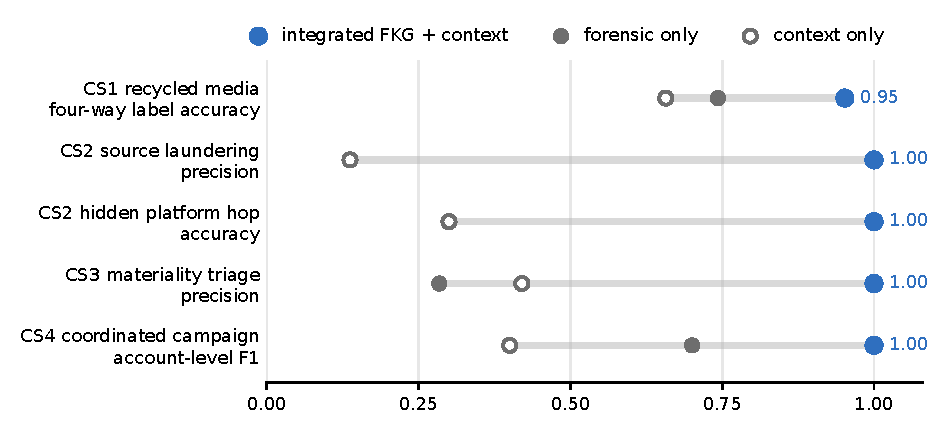
\includegraphics[width=\linewidth]{figures/headline.pdf}
\caption{Headline results, one row per investigative question. Section 5 gives each study's setup; section 6 shows how the gaps hold under noise.}
\end{figure}
\textbf{Five}\textbf{ things to take away}

\begin{itemize}
\item \textbf{The gain comes from integration, not detection.} Every arm of every study reads the same detector outputs; only the joins differ. The forensic layer alone cannot see time, claims or accounts, and the context layer alone cannot see what was altered.
\item \textbf{Errors are misses, not false accusations.} Joins rarely invent evidence, so noise lowers recall while precision holds: 1.00 at every noise rate for CS3 triage, at least 0.81 for CS1 recycled-media flags up to η = 0.5.
\item \textbf{Defence is a new query, not a new model.} In the campaign study, each attack that broke detection was answered by a new query over the same records (of seventeen attacks, seven fixed, four partly, six open). This is the empirical case for FKG as a living system rather than a fixed detector.
\item \textbf{Forensic TTPs outlast personas.} When operators retire every account after each wave, the processing-chain join still links 85\% of new waves to the right operator and none to the wrong one, where account overlap links none and narrative or timing name the wrong operator in 12 to 62\% of waves. It holds over a simulated year (4.8M quads) and against 23 benign look-alike accounts per campaign account; within-wave precision is what the base rate erodes.
\item \textbf{The schema is enough for agents.} Agents given only a page of data notes wrote correct investigative SPARQL (held-out mean 0.92 to 0.96 against 0.91 by hand). This is what makes FKG usable by analysts who do not write queries.
\end{itemize}
\section*{2. How it fits together}
\begin{figure}[tbp]\centering
% Architecture of the proposal: the FKG record joined to four context layers by shared identifiers.
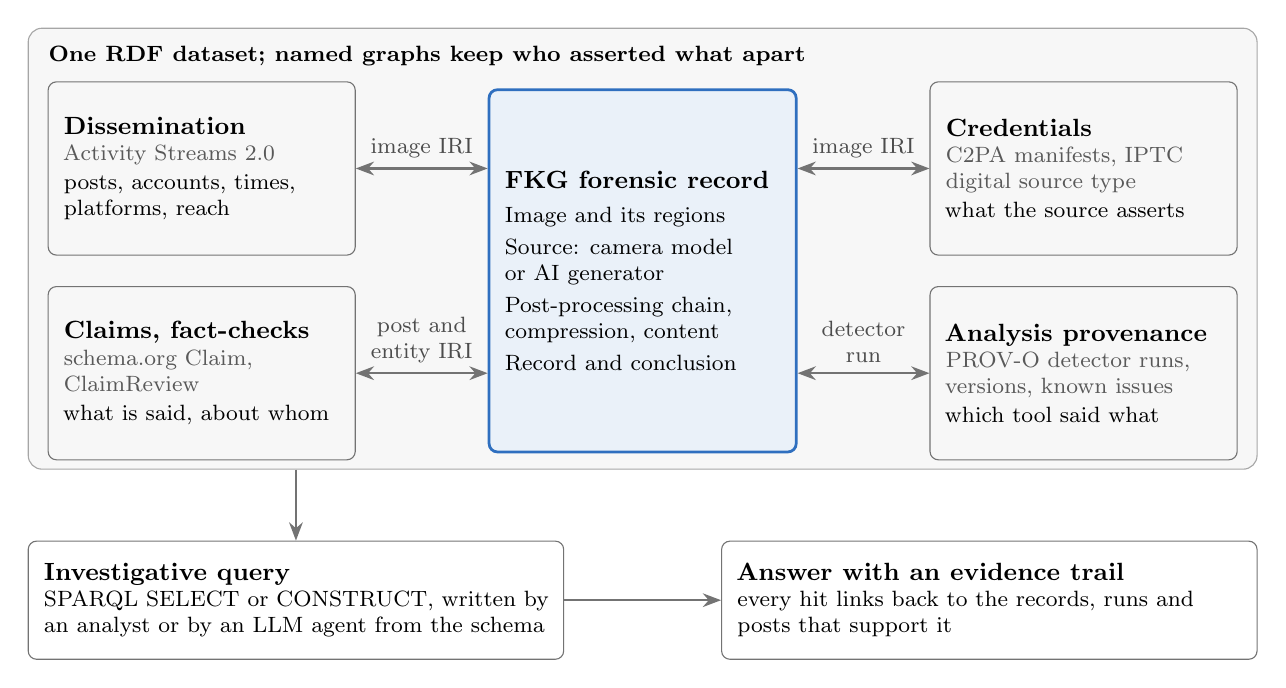
\begin{tikzpicture}[
  font=\footnotesize, >=Stealth,
  box/.style={draw=black!55, rounded corners=3pt, minimum width=3.9cm, align=flush left, inner sep=5pt, text width=3.5cm, font=\footnotesize},
  main/.style={box, draw=fkgblue, fill=fkgblue!10, line width=1pt},
  head/.style={font=\small\bfseries},
  std/.style={font=\footnotesize\color{black!65}},
  key/.style={font=\footnotesize\color{black!70}, align=center},
  link/.style={<->, draw=black!55, thick}]
  \node[main, minimum height=4.6cm] (fkg) at (0,0) {{\small\bfseries FKG forensic record}\\[3pt]
    Image and its regions\\[2pt] Source: camera model\\ or AI generator\\[2pt] Post-processing chain,\\ compression, content\\[2pt] Record and conclusion};
  \node[box, minimum height=2.2cm] (dis) at (-5.6, 1.3) {{\small\bfseries Dissemination}\\ {\footnotesize\color{black!65}Activity Streams 2.0}\\[1pt] posts, accounts, times, platforms, reach};
  \node[box, minimum height=2.2cm] (cla) at (-5.6,-1.3) {{\small\bfseries Claims, fact-checks}\\ {\footnotesize\color{black!65}schema.org Claim, ClaimReview}\\[1pt] what is said, about whom};
  \node[box, minimum height=2.2cm] (cre) at ( 5.6, 1.3) {{\small\bfseries Credentials}\\ {\footnotesize\color{black!65}C2PA manifests, IPTC digital source type}\\[1pt] what the source asserts};
  \node[box, minimum height=2.2cm] (pro) at ( 5.6,-1.3) {{\small\bfseries Analysis provenance}\\ {\footnotesize\color{black!65}PROV-O detector runs, versions, known issues}\\[1pt] which tool said what};
  \draw[link] (dis.east) -- node[key, above] {image IRI} (dis.east -| fkg.west);
  \draw[link] (cla.east) -- node[key, above] {post and\\entity IRI} (cla.east -| fkg.west);
  \draw[link] (cre.west) -- node[key, above] {image IRI} (cre.west -| fkg.east);
  \draw[link] (pro.west) -- node[key, above] {detector\\run} (pro.west -| fkg.east);
  \begin{scope}[on background layer]
    \node[draw=black!35, fill=black!3, rounded corners=5pt, inner sep=7pt, fit=(dis)(cla)(cre)(pro)(fkg), yshift=8pt, minimum height=5.6cm] (ds) {};
  \end{scope}
  \node[font=\footnotesize\bfseries, anchor=north west] at ([xshift=4pt,yshift=-3pt]ds.north west) {One RDF dataset; named graphs keep who asserted what apart};
  \node[box, text width=6.4cm, minimum width=6.8cm, minimum height=1.5cm, anchor=north west] (q) at ([yshift=-0.9cm]ds.south west) {{\small\bfseries Investigative query}\\ SPARQL SELECT or CONSTRUCT, written by an analyst or by an LLM agent from the schema};
  \node[box, text width=6.4cm, minimum width=6.8cm, minimum height=1.5cm, anchor=north east] (a) at ([yshift=-0.9cm]ds.south east) {{\small\bfseries Answer with an evidence trail}\\ every hit links back to the records, runs and posts that support it};
  \draw[->, draw=black!55, thick] (q.north |- ds.south) -- (q.north);
  \draw[->, draw=black!55, thick] (q.east) -- (a.west);
\end{tikzpicture}

\caption{Architecture. The FKG record is unchanged from [1]; everything around it reuses an existing standard. Labels on the arrows are the join keys.}
\end{figure}
\begin{itemize}
\item \textbf{The forensic layer is FKG as published} [1]: per image, regions, each region's source (camera model or AI generator, with confidence), the post-processing chain, compression and depicted content, rolled up into a record and conclusion. We add nothing to its semantics.
\item \textbf{The context layer is mostly borrowed.} Posts and accounts are Activity Streams 2.0, claims and verdicts are schema.org Claim and ClaimReview, credentials summarise C2PA manifests with IPTC source types, and detector runs are PROV-O activities. The new vocabulary is a handful of terms (for example a post's platform, a platform's transcoding profile, a known detector issue).
\item \textbf{Three identifiers do the joining}: the image IRI (shared by the post that attaches it, its credential and its FKG record), the entity IRI (shared by a claim's subject and the content FKG says was altered) and the detector run (shared by the record and the fact-check that cites it).
\item \textbf{Named graphs record who asserted what}, so a query can trust the detector but not the uploader, or ask which conclusions rest only on a publisher's own credential.
\item \textbf{SHACL validates every record}; the competency questions run as plain SPARQL 1.1 with no reasoner.
\end{itemize}
\section*{3. What is new}
\textbf{Novelty in one sentence:} forensic observations become first-class linked data, so an investigation is a composition of standard queries over shared identifiers rather than a bespoke pipeline per question.

\begingroup\small
\begin{xltabular}{\linewidth}{@{\extracolsep{0pt plus 1fil}}>{\raggedright\arraybackslash\hsize=0.9093\hsize}X>{\raggedright\arraybackslash\hsize=0.9631\hsize}X>{\raggedright\arraybackslash\hsize=1.0063\hsize}X>{\raggedright\arraybackslash\hsize=1.1213\hsize}Xl@{}}
\toprule
\textbf{Line of work} & \textbf{What it gives} & \textbf{What it cannot do alone} & \textbf{What FKG as linked data adds} & \textbf{Shown in} \\
\midrule
\endhead
FKG [1] & An explainable forensic record per image & Nothing about posts, claims, time or other images & The same record, joinable across images, posts and claims & all \\
Content credentials (C2PA, IPTC) [7, 8] & Signed provenance asserted by the publisher & An assertion, not an observation; stripped on re-upload; can be wrong & Assertions checked against forensic observations & CS3 \\
Image provenance analysis [11] & Near-duplicate graphs from pixel similarity & Edge direction and what each edit did stay ambiguous; no claims or accounts & Copies ordered by forensic traces (compression, resampling, inserted regions) and tied to posts and accounts & CS2 \\
Out-of-context detection [10] & Image and caption mismatch from learned embeddings & No time, no earliest appearance, no evidence trail & Recycled media as a temporal join over claims, events and first appearance & CS1 \\
Fact-check data (ClaimReview) [6] & Verdicts linked to claims & Verdicts are not linked to the evidence or the tool version behind them & Verdict to record to detector run, so a detector bug has a queryable blast radius & CS3 \\
Coordinated behaviour detection [12] & Co-posting and co-sharing networks & Flags sincere believers; misses operations that share a toolchain but not content & A forensic TTP join (same generator and processing recipe) combined with narrative and timing & CS4 \\
Threat intelligence (STIX, DISARM) [13, 14] & Vocabulary for tactics, techniques and campaigns & TTPs are entered by analysts, not inferred from the media & TTPs inferred from forensic records, ready to export (proposed, not built) & — \\
\bottomrule
\end{xltabular}
\endgroup

\textbf{Why it should get published:} each row above is an established community whose artefacts FKG can now join, and every join is shown to matter on a measurable task. The paper's contribution is the bridge, the competency questions that exercise it, and evidence that both hand-written and agent-written queries can use it.

\section*{4. Use-case landscape}
Eighteen use cases fall into four families. Twelve are scored in the case studies; six have sketch queries only (full catalog in Appendix A).

\begingroup\small\par\smallskip\noindent
\begin{tabularx}{\linewidth}{@{\extracolsep{0pt plus 1fil}}>{\raggedright\arraybackslash\hsize=0.6181\hsize}X>{\raggedright\arraybackslash\hsize=1.1086\hsize}X>{\raggedright\arraybackslash\hsize=1.4792\hsize}X>{\raggedright\arraybackslash\hsize=1.0514\hsize}X>{\raggedright\arraybackslash\hsize=0.7427\hsize}X@{}}
\toprule
\textbf{Family} & \textbf{Question it answers} & \textbf{Use cases} & \textbf{Context it needs} & \textbf{Evidence} \\
\midrule
\textbf{Time and origin} & When did this first appear, and is it presented as something it predates? & UC1 recycled media, UC2 earliest appearance, UC10 anachronistic attribution & Posts and timestamps, events, generator release dates & CS1, CS3 \\
\textbf{Copies and lineage} & How did this file travel and change, and who changed it? & UC3 patient zero, UC4 lineage, UC5 source laundering, UC6 hidden platform hop, UC13 toolkit fingerprint, UC14 shared device & Posts, accounts, platform transcoding profiles & CS2 (UC3 to UC6); UC13 and UC14 sketched \\
\textbf{Claims and intent} & Does the alteration matter for what is claimed, and who is pushing it? & UC7 materiality, UC8 credential contradiction, UC9 presentation and intent, UC12 coordinated campaign, UC17 generator exposure & Claims and their subjects, disclosures, credentials, accounts & CS3 (UC7 to UC9), CS4 (UC12); UC17 sketched \\
\textbf{Auditing the analysis} & Which conclusions rest on which evidence, and what changes when a detector is wrong? & UC11 recall impact, UC15 detector consistency, UC16 audit trail, UC18 reported versus inferred & Detector runs and versions, ClaimReview, credentials & CS3 (UC11); others sketched \\
\bottomrule
\end{tabularx}
\par\medskip\endgroup

The first three families are what an investigator asks; the fourth is what an auditor or a court asks of the investigation itself. The fourth is where an explicit, queryable record of analysis provenance has no substitute, and it is the least developed here.

\section*{5. Case studies}
Each study plants ground truth in a seeded synthetic world and scores the integrated query against a \textbf{forensic-only} baseline (the FKG layer alone), a \textbf{context-only} baseline (posts, time, credits, claims) and \textbf{ablations} that remove one FKG-based guard. The worlds also plant the failures a real pipeline has: detector false positives and weak true positives near the 0.7 confidence threshold, near-duplicate clusters that wrongly merge different photos, and an incomplete crawl.

\begingroup\small\par\smallskip\noindent
\begin{tabularx}{\linewidth}{@{\extracolsep{0pt plus 1fil}}l>{\raggedright\arraybackslash\hsize=0.9603\hsize}X>{\raggedright\arraybackslash\hsize=1.0579\hsize}X>{\raggedright\arraybackslash\hsize=0.8851\hsize}X>{\raggedright\arraybackslash\hsize=1.0967\hsize}X@{}}
\toprule
 & \textbf{CS1} & \textbf{CS2} & \textbf{CS3} & \textbf{CS4} \\
\midrule
Scenario & Claim posts about two current events & Eight outlet photos spreading across five platforms & Posts about five public figures, some altered & A flood-rumour influence operation \\
Size & 105 claim posts, 63 accounts, 10k quads & 241 image instances, 6 AI edits & 204 posts, 68 accounts & 168 accounts, about 770 posts and 650 images \\
Use cases & UC1, UC2 & UC3 to UC6 & UC7 to UC11 & UC12 \\
\bottomrule
\end{tabularx}
\par\medskip\endgroup

\subsection*{CS1. Recycled media: is an authentic photo presented as showing an event it predates?}
\begin{itemize}
\item \textbf{Why one layer fails.} The photo is forensically clean, so the forensic layer cannot flag it (recycled-class F1 0). Context alone is fooled when near-duplicate clustering merges a current photo with an old one.
\item \textbf{The join.} Flag a post whose image has no reliable AI region and whose near-duplicate cluster holds a copy published before the claimed event's start date \textbf{and attributed to the same camera model}. That camera-agreement guard defeats false merges.
\end{itemize}
\begingroup\small\par\smallskip\noindent
\begin{tabularx}{\linewidth}{@{\extracolsep{0pt plus 1fil}}>{\raggedright\arraybackslash\hsize=1.0976\hsize}X>{\raggedright\arraybackslash\hsize=0.9024\hsize}Xll@{}}
\toprule
\textbf{Measure} & \textbf{Integrated} & \textbf{Forensic only} & \textbf{Context only} \\
\midrule
Recycled posts flagged (CQ1.1) & P 1.00, R 0.88 & F1 0 & — \\
Earliest appearance found (CQ1.2) & 22 of 22 & — & — \\
Four-way label accuracy (CQ1.3) & \textbf{0.952} & 0.743 & 0.657 \\
Ablations (accuracy) & no camera guard 0.924; no confidence threshold 0.943 &  &  \\
\bottomrule
\end{tabularx}
\par\medskip\endgroup

\textbf{Takeaway.} The recall ceiling of 0.88 is the open world made visible: three recycled photos have no pre-event copy in the crawl, and the graph declines to guess rather than accuse.

\subsection*{CS2. Lineage and laundering: which copy added the synthetic region, and who is misattributing it?}
\begin{itemize}
\item \textbf{Why one layer fails.} Timestamps order copies but cannot say which one changed the content. Forensic records describe each file but not who posted it, where, or whom it credits.
\item \textbf{The joins.}

\begin{itemize}
\item \emph{Lineage} is two CONSTRUCT rules. The first proposes earlier copies in the same cluster that satisfy forensic monotonicity (AI regions survive, resolution never grows, a pass-through keeps its compression). The second picks one by parsimony and writes prov:wasDerivedFrom plus the edit step.
\item \emph{Laundering}: the post credits an outlet, the generator and content pair is corroborated, and the outlet never posted that pair.
\item \emph{Hidden hop}: a pass-through file's quality factor is matched to the platforms' transcoding profiles.
\end{itemize}
\end{itemize}
\begingroup\small
\begin{xltabular}{\linewidth}{@{\extracolsep{0pt plus 1fil}}>{\raggedright\arraybackslash\hsize=0.9724\hsize}X>{\raggedright\arraybackslash\hsize=0.7500\hsize}X>{\raggedright\arraybackslash\hsize=1.2776\hsize}X@{}}
\toprule
\textbf{Measure} & \textbf{Integrated} & \textbf{Best baseline} \\
\midrule
\endhead
Hidden platform hop (CQ2.4) & \textbf{50 of 50} & previous post's platform: 15 of 50 \\
Laundering (CQ2.3) & \textbf{P 1.00, R 1.00} & every outlet-crediting post: P 0.137 \\
Lineage, parent in the right variant (CQ2.2) & 1.000 & timestamps only: 0.893 \\
Lineage, exact parent & 0.288 & timestamps only: 0.176 \\
Edit steps found & 6 of 6, P 0.86 & not expressible without forensics \\
Patient zero (CQ2.1) & P 0.75, R 0.50 (F1 0.56 over 10 seeds) & earliest post in cluster: 0 \\
\bottomrule
\end{xltabular}
\endgroup

\textbf{Takeaway.} Forensic traces orient the copy graph that pixel similarity leaves undirected. Patient zero is the weak spot: a content-driven detector error recurs on copies, so recurrence is weak evidence that an edit is real. Agents found a sharper cue (§7).

\subsection*{CS3. Materiality and intent: does the alteration matter for what is claimed, and was it disclosed?}
\begin{itemize}
\item \textbf{Why one layer fails.} Forensics alone queues every AI-altered post, including disclosed art and sky replacements (precision 0.284). Context alone queues every undisclosed claim post, altered or not (0.420).
\item \textbf{The join.} The altered region's content links to \textbf{the same entity IRI the claim is about}, and nothing discloses it (no platform label, caption or credential). A CONSTRUCT rule writes the presentation category back as an inferred conclusion with its provenance.
\item \textbf{Auditing the analysis.} Credentials are checked against forensics; attributions are checked against generator release dates; fact-checks are traced through their record to the detector version and its known issue.
\end{itemize}
\begingroup\small
\begin{xltabular}{\linewidth}{@{\extracolsep{0pt plus 1fil}}>{\raggedright\arraybackslash\hsize=1.4196\hsize}X>{\raggedright\arraybackslash\hsize=0.5804\hsize}Xll@{}}
\toprule
\textbf{Measure} & \textbf{Integrated} & \textbf{Forensic only} & \textbf{Context only} \\
\midrule
\endhead
Triage queue precision (CQ3.1) & \textbf{1.00} at recall 0.912 & 0.284 & 0.420 \\
Same, without the materiality join & 0.646 &  &  \\
Presentation category accuracy (CQ3.3) & \textbf{0.971} & 0.603 & 0.740 \\
Credentials contradicted by forensics (CQ3.2) & 8 of 8 &  &  \\
Attributions to an unreleased generator (CQ3.4) & 3 of 3 &  &  \\
Fact-checks resting on the faulty detector (CQ3.5) & 5 of 5 &  &  \\
\bottomrule
\end{xltabular}
\endgroup

\textbf{Takeaway.} Materiality is the whole effect, and it needs one shared entity IRI. “Intent” is deliberately modest: the graph infers how content was presented, which is evidence about intent, not intent.

\subsection*{CS4. Coordinated campaign: which accounts run a manipulated-media operation? (companion study)}
Run as a separate, deeper study; full write-up and code in the repository's \href{https://github.com/ductai199x/fkg-case-studies/tree/main/coordinated-campaign}{\code{coordinated-campaign/}} folder.

\begin{itemize}
\item \textbf{Why one layer fails.} The world hides 12 operator accounts among decoys that each defeat one signal. Forensics alone flags a brand campaign that also runs one image pipeline (F1 0.70). Claims and timing alone flag 20 sincere believers (precision 0.25, F1 0.40).
\item \textbf{The join, one SPARQL query.} A forensic TTP match (same generator, at least two processing operations with parameters within 15\%), not a re-upload, a shared fact-checked false claim, and a 72-hour window. A second hop adds the two text-only amplifiers.
\end{itemize}
\begin{figure}[tbp]\centering
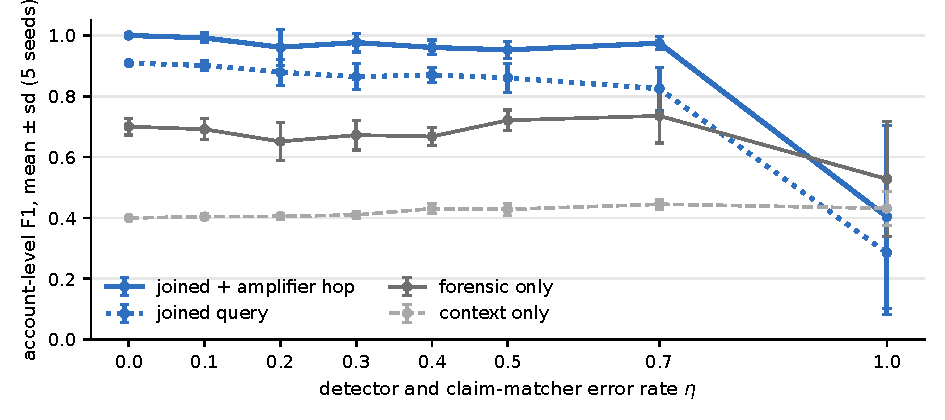
\includegraphics[width=\linewidth]{figures/campaign_noise.pdf}
\caption{CS4 results from the companion study. Here η is the error rate of detectors and claim matchers, not the per-failure rate used in CS1 to CS3. At η = 1.0 detector output is mostly noise and every forensic query collapses, as it should.}
\end{figure}
\begin{itemize}
\item \textbf{Agents rediscovered the join.} Three LLM investigators given only a schema card and the analyst's question each found exactly the 12 accounts and independently wrote the same forensic-and-claim rule. Detectors written from noisy data reach F1 0.92 and 0.94 at η = 0.7 on held-out worlds; the one written from clean data is too strict (0.31).
\item \textbf{Eight rounds of attack and defence}, in single-event worlds up to 30× larger (745k quads), over a simulated year of waves (up to 4.84M quads), and calibrated to published measurements. Every defence is a new query over the same records:
\end{itemize}
\begingroup\small
\begin{xltabular}{\linewidth}{@{\extracolsep{0pt plus 1fil}}>{\raggedright\arraybackslash\hsize=1.2608\hsize}X>{\raggedright\arraybackslash\hsize=0.5478\hsize}X>{\raggedright\arraybackslash\hsize=1.1914\hsize}Xl@{}}
\toprule
\textbf{Attack (F1 at η = 0.3 unless stated)} & \textbf{What broke} & \textbf{Defender's new query} & \textbf{After} \\
\midrule
\endhead
Per-persona processing presets & joined query 0.05 & self-consistent processing per account & 0.78 \\
30× organic population & precision 0.37 & gate on self-consistency & precision 1.0 \\
Five calibrated realism models at once & 0.63 & open-world: claim need only be not rated true & 0.76 \\
Debunkers repost campaign images & precision 0.70 & stance filter on claim links & precision 0.93 \\
One or two posts per persona & at most 0.34 & union with a behavioural rule & 0.63 \\
Per-persona processing on aged accounts & 0.02 & repost ties plus an age-free amplifier hop & 0.59 \\
Operator also stops reposting its personas & 0.26 & one agreeing operation suffices & 0.42 \\
Full account turnover between waves & overlap links 0\% of waves & cross-wave TTP join, chained labels & 85\% right, 0\% wrong \\
Two operators buy the same toolkit & 32\% wrong links & keep FKG labels that narrative or timing confirm & 22\% wrong \\
Platform-scale query cost & over 30 min at 1.09M quads & scope each query to the event window & 30 s at 1.46M quads \\
23 benign look-alikes per campaign account & precision 0.41 & house-style tenure & precision 0.55 \\
Random processing per image; 12-day spread; a fresh pipeline per persona each wave; 10× population through the amplifier hop; 60-day persona warm-up &  &  & open \\
\bottomrule
\end{xltabular}
\endgroup

\begin{itemize}
\item \textbf{Detection is evidence-limited.} All campaign accounts have acted by 24 hours, yet the best F1 at η = 0.3 is 0.36 at 24 hours and 0.53 at 36 hours, because personas need time to post two matching images.
\end{itemize}
\subsection*{CS4, long horizon: does the forensic TTP link a new wave to a known operator, months later?}
Real operators run campaigns in waves, retire their personas after each one and change tools, while platforms name an operator only weeks later in a takedown report. So a new wave arrives from accounts that share nothing with the old ones except, possibly, how their images were made.

\begin{itemize}
\item \textbf{The world.} Six news events four weeks apart (twelve for the one-year runs). Two operators each run one wave per event with fresh personas (16 and 11 accounts), retire them, and drift their processing presets (5\% per wave, a 15\% chance of swapping a tool). Takedown reports name the operator for 80\% of waves, list 75\% of its accounts and arrive a median 35 days late. 450 organic accounts, fan groups, brand agencies and debunkers share the platform, with every realism model of the stress rounds switched on.
\item \textbf{The cross-wave query.} A post in the current event window with a synthetic image and an unrefuted claim is matched to an earlier account that a takedown names or an earlier wave flagged, using the same TTP test (at least two operations with parameters within 15\%). Labels are read off the takedown report directly or by following such links back through earlier waves (chained, at most six hops).
\item \textbf{Every snapshot is the graph as it stood 96 hours after the event began}, built only from records visible by then, so nothing from the future leaks in.
\end{itemize}

\textbf{Finding 1: FKG links new waves to the right operator and almost never to the wrong one.} Pooled over events 2 to 6, three seeds and two noise levels (60 operator waves per world), the chained FKG link is right for 85\% of waves and wrong for none in the base world. Account overlap and co-repost similarity link 0\%, because fresh personas share no accounts. Narrative and timing link about as often but are wrong for 12\% and 28\% of waves, and collapse when operators push the same narratives (62\% wrong) or use a scheduling tool (50\% wrong). Chaining through earlier waves beats the one-hop link on held-out seeds (82\% against 72 to 75\%).

\begin{figure}[tbp]\centering
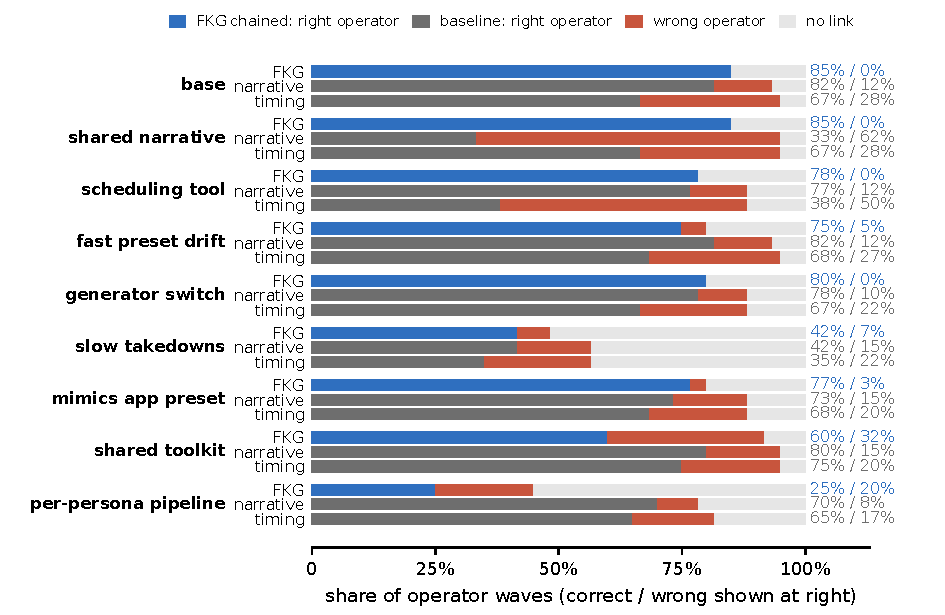
\includegraphics[width=\linewidth]{figures/waves_links.pdf}
\caption{Cross-wave attribution under attack. Each bar is the share of operator waves (events 2 to 6, three seeds, $\eta \in \{0, 0.3\}$) whose flagged accounts are labelled with the right operator, the wrong one, or not at all. FKG uses the chained forensic link; the baselines label by narrative topics and posting hours learned from takedown reports. Account overlap and co-repost similarity link no wave in any world and are omitted.}
\end{figure}

\textbf{Finding 2: what breaks it is shared or per-persona processing, not time.} Per-persona pipelines leave nothing to match (25\% right, 20\% wrong). Two operators buying the same toolkit makes them indistinguishable (32\% wrong). Slow, sparse takedowns starve every method equally (about 42\%). Requiring narrative or timing to agree with the FKG label keeps the wrong-link rate at or below 7\% wherever FKG works, at the cost of recall.

\textbf{Finding 3: queries scale if they are scoped to the event.} Over a year of events the graph grew from 73k to 1.46M quads (1x population) and from 220k to 4.84M quads (10x population, 1,900 accounts).
\begingroup\small\par\smallskip\noindent
\begin{tabularx}{\linewidth}{@{}>{\raggedright\arraybackslash}X r r r r@{}}
\toprule
\textbf{Joined detection query} & \textbf{1x, event 2} & \textbf{1x, event 12} & \textbf{10x, event 2} & \textbf{10x, event 12} \\
\midrule
Graph size (quads) & 191k & 1.46M & 621k & 4.84M \\
Unscoped, whole history & 11 s & over 30 min & 144 s & over 5 min (limit) \\
Scoped to the event window & 1.4 s & 30 s & 14 s & 163 s \\
Window-only store (identical answers) & 0.4 s & 0.5 s & 4.5 s & 3.5 s \\
Cross-wave TTP edges & 0.1 s & 0.9 s & 0.2 s & 6.0 s \\
\bottomrule
\end{tabularx}
\par\medskip\endgroup
The unscoped query passed 30 minutes at 1.09M quads. A store that holds only the current window (about 30k quads at 1x, 100k at 10x) answers the joined query in seconds with identical results at every event, so an incremental deployment is feasible. The repost-tie query needs about two weeks of look-back, not just the window, and is the slowest step on the full graph (up to 25 minutes at 3.2M quads). Cross-wave links stay right as the graph grows: 18 of 22 operator waves at 1x and 19 of 22 at 10x, with at most one wrong; the misses are abstentions before the first takedown reports appear.

\textbf{Finding 4: the base rate of benign coordination is the real limit, and generator identity is what holds.} Fan groups that pass a false claim around in one house style, brand agencies running cause-marketing posts, and news outlets syndicating one wire image through a shared CMS pipeline were added on top of the base world, up to 23 look-alike accounts per campaign account (Figure~\ref{fig:wscale}b; three seeds, $\eta \in \{0, 0.3\}$, a noise-only redraw as control).
\begin{itemize}
\item \textbf{Within-wave detection precision falls from 0.87 to 0.41} while recall stays near 0.65; a redraw of the noise alone moves it by 0.06. Fans cause 81\% of the false positives: within one event they are a small, sincere campaign. Brand and news posts rarely trip it, because true claims get rated and syndicated copies carry provenance.
\item \textbf{Operator-wave links stay right.} The chained FKG link was never wrong at any ratio. At the account level, attribution precision holds best when the generator must match (0.90 to 0.72), against 0.54 for any generator, 0.35 for narrative and 0.28 for timing.
\item \textbf{Population growth hits a different step.} At 10x population the core joined query keeps precision 0.69, but the amplifier hop pulls in organic accounts that reposted campaign posts (570 of 581 false positives), so the flagged set's precision falls to 0.30.
\item \textbf{A new query recovers part of it: house-style tenure.} Dropping candidates whose window images match two or more of their own images posted more than 30 days earlier raises precision from 0.60 to 0.72 at 8 look-alikes per campaign account and from 0.38 to 0.55 at 23, and drops no campaign account. Fans who only repost inside their group are untouched (311 of 675 fan false positives remain).
\item \textbf{The operator can buy its way past tenure.} Personas that post the wave's kit style weekly for 60 days before the wave get dropped by the filter (188 campaign accounts), and recall falls from 0.63 to 0.43. Tenure therefore raises the cost of a wave, from three weeks of persona upkeep to two months, rather than closing the gap. The cross-wave link is unaffected (85\% right, at most 2\% wrong).
\end{itemize}

\begin{figure}[tbp]\centering
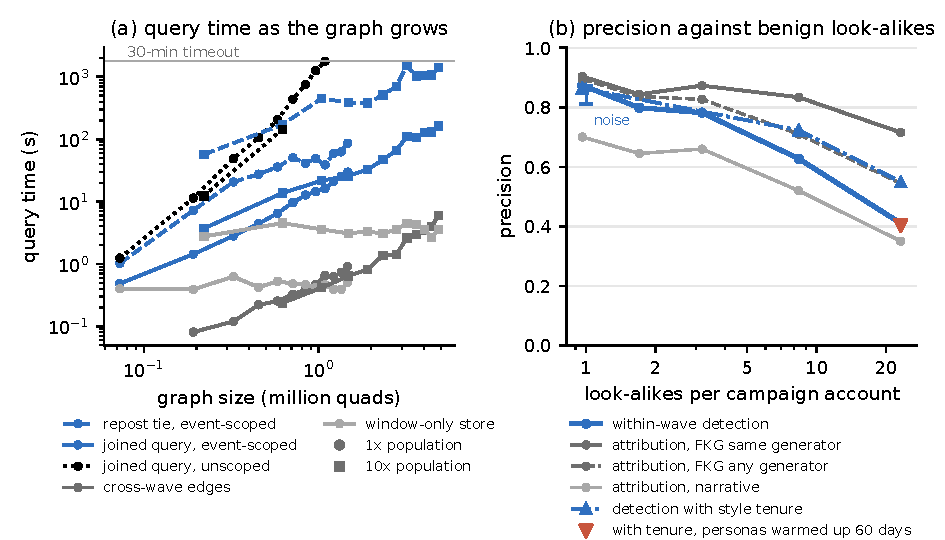
\includegraphics[width=\linewidth]{figures/waves_scale.pdf}
\caption{(a) Query time against graph size over twelve monthly events, at 1x and 10x population; the unscoped query stops at its timeout. (b) Precision against the number of benign look-alike accounts (fans, brand agencies, news syndicators) per campaign account, events 2 to 6 pooled over three seeds and $\eta \in \{0, 0.3\}$. The bar at 1 is the spread between two draws of observation noise on the same world. The tenure curve comes from a rerun with four months of platform history before the first event.}\label{fig:wscale}
\end{figure}

\textbf{Takeaway.} The forensic records carry the evidence that is hardest for an operator to remove, and every attack was met by a query, not a retrained model. Over months, the same records link new waves to known operators where account, repost, narrative and timing signals fail, and they stay right as the graph grows and benign look-alikes multiply; what falls is within-wave precision, which is a base-rate problem the paper should state plainly. The paper should claim that the join \textbf{raises the cost of running a campaign} (a shared toolkit, per-persona pipelines or two months of persona warm-up are what it takes to evade it) and finds it as it completes, not that it cannot be evaded.

\section*{6. Robustness to noise}
The single-seed tables fix the number of planted failures, so each CS1 and CS3 world was regenerated with every failure mode at rate η (five seeds per rate). CS2 was rerun over ten fresh seeds, since its spread trees already vary by seed.

\begin{figure}[tbp]\centering
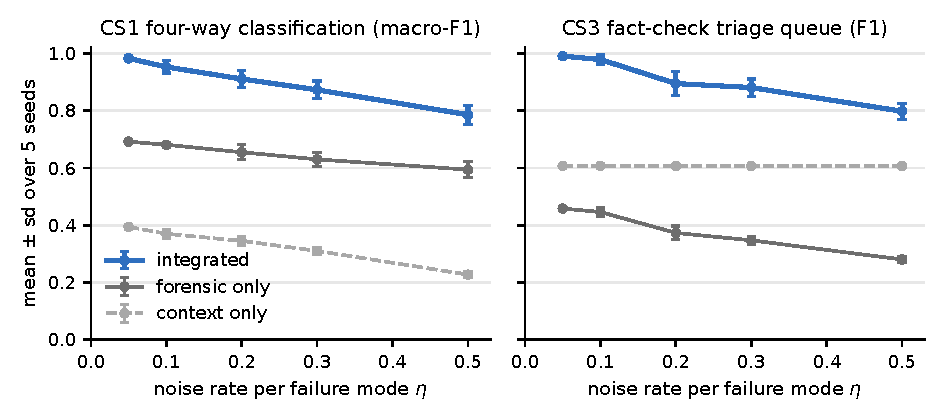
\includegraphics[width=\linewidth]{figures/noise_sweep.pdf}
\caption{Noise sweep for CS1 and CS3. Every failure mode (detector false positives, a quarter above threshold; weak true positives; false cluster merges; missing earliest appearances) is drawn independently at rate η.}
\end{figure}
\begin{itemize}
\item \textbf{The ordering never flips.} At η = 0.5, where half of all items carry a failure, CS1 still reaches 0.786 against 0.594 for forensics alone, and the CS3 queue 0.798 against 0.607 for context alone.
\item \textbf{Noise costs recall, not precision.} CS3 triage precision is exactly 1.00 at every rate while recall falls from 0.983 to 0.665; CS1 recycled-media precision stays at or above 0.81.
\item \textbf{FKG guards matter more as noise grows.} Without the camera-agreement guard, CS1 accuracy is 0.766 instead of 0.882 at η = 0.3, and 0.615 instead of 0.804 at η = 0.5.
\item \textbf{CS2 over ten seeds.} Parent in the right variant 0.994, laundering F1 0.96 (precision 0.98), hidden hops 1.00 in every seed; patient zero F1 0.56 ± 0.17 at precision 0.905, its variance being how many edits happen to spread.
\item \textbf{What the sweep does not show.} The CS3 context-only line is flat because no noise touches context, and the credential, anachronism and recall-impact queries stay at 1.00 because nothing they read is perturbed. That is a property of the sweep, not evidence of robustness.
\end{itemize}
\section*{7. Agentic investigation}
Can an LLM agent turn an investigator's question into correct SPARQL from the schema alone? Each agent received the 12 natural-language questions of CS1 to CS3, the two ontology files and one page of data notes, with no queries and no hint of the hand-written rules.

\begingroup\small\par\smallskip\noindent
\begin{tabularx}{\linewidth}{@{\extracolsep{0pt plus 1fil}}l>{\raggedright\arraybackslash\hsize=1.0000\hsize}X@{}}
\toprule
\textbf{Arm} & \textbf{What it could see} \\
\midrule
Hand-written & everything (written by the study author) \\
A1, A2 & questions, ontology, notes; no data (tested on toy graphs they built) \\
B1, B2 & the same, plus query access to the three worlds \\
B1r, B2r & as B1 and B2, fresh agents run after the leak fix \\
\bottomrule
\end{tabularx}
\par\medskip\endgroup

\begin{figure}[tbp]\centering
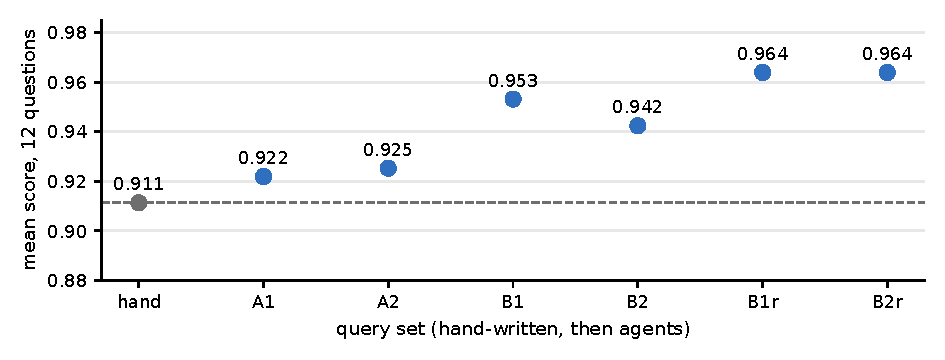
\includegraphics[width=\linewidth]{figures/agents_heldout.pdf}
\caption{Agent and hand-written query sets, mean over the 12 questions of CS1 to CS3. The dashed line marks the hand-written held-out mean. Per-question scores are in Appendix D.}
\end{figure}
\begin{itemize}
\item \textbf{Agents match or beat hand-written queries} on held-out worlds (0.922 to 0.964 against 0.911). Every agent found the guards the hand-written queries rely on: camera agreement, the reliability threshold, the entity-to-claim join and the walk from fact-check to detector version.
\item \textbf{Three agent ideas are worth adopting.} Treating an attribution seen only on a cluster's earliest copy as a detector error (patient zero 0.545 to between 0.875 and 0.933). A single-compression cue for pasted regions (patient zero and laundering 1.00; an upper bound, since the simulator records that trace without noise). Checking the resampling scale between parent and child (exact parent 0.299 to 0.456).
\item \textbf{Where agents did worse, the cause was the question or the access.} A1 and A2 read an underspecified credential question differently (0.762). A1's lineage query is correct but takes 540 to 800 seconds; without data access an agent cannot see that a query is too slow.
\item \textbf{An agent found a flaw in our simulator.} B2 noticed that planted false positives were separable from real ones, which exposed a label leak in the first generators (Appendix C). Agents as auditors of synthetic benchmarks is a small result in its own right.
\item \textbf{In CS4,} three investigators given only a schema card recovered the campaign join unaided (§5).
\end{itemize}
\section*{8. Encoding decisions for Jane}
CS1 to CS3 and CS4 were built in parallel and made different, reversible choices. The paper needs one answer per row.

\begingroup\small
\begin{xltabular}{\linewidth}{@{\extracolsep{0pt plus 1fil}}l>{\raggedright\arraybackslash\hsize=0.6816\hsize}X>{\raggedright\arraybackslash\hsize=1.2260\hsize}X>{\raggedright\arraybackslash\hsize=1.0228\hsize}X>{\raggedright\arraybackslash\hsize=1.0696\hsize}X@{}}
\toprule
\textbf{\#} & \textbf{Decision} & \textbf{CS1 to CS3} & \textbf{CS4} & \textbf{Question for Jane} \\
\midrule
\endhead
1 & Where new terms live & All new terms in a separate ctx: vocabulary; nothing added to fkg: & One new fkg: term (FullySynthetic) & Should the context vocabulary join FKG 0.2, or ship as a profile that imports it? \\
2 & Fully synthetic images & ctx:SyntheticImage & fkg:FullySynthetic as a manipulation type & A verdict value, a manipulation type, or both? \\
3 & Named graphs & One per forensic record, plus reference and context graphs & One per producer (forensics, platform, fact-check, provenance) & Per record (fine-grained provenance), per producer (simple trust policies), or both? \\
4 & Observation layer & Keeps the record layer (record, conclusion, verdict, evidence status, limitation note); no per-assertion observations & Drops evidence status and limitation note; one PROV activity per image; adds localization status & Named graphs or RDF 1.2 triple terms for statement-level provenance? Must the paper keep per-observation nodes? \\
5 & Image identifiers & example.org IRIs & Content-derived ni:///sha-256 IRIs (RFC 6920) & Adopt content-derived IRIs, which make the join key independent of any platform? \\
6 & Compression & Node typed both LastCompressed and ReCompressed, plus a boolean & ReCompressed plus a boolean & Are the two subclasses disjoint? If so, keep only the boolean. \\
7 & Entity links from content & ctx:depictsEntity IRI beside the free-text description & Free text only & Should Content carry entity IRIs natively, ideally to an external KG? CS3 depends on it. \\
8 & Axioms SHACL cannot check & Functional source, disjointness and cardinalities checked; Axiom 1 (regions partition the image) and Axiom 4 (causal order) not & Same & Region masks for Axiom 1? SHACL-SPARQL for Axiom 4? \\
9 & Reliability threshold & 0.7 hard-coded in every query & Thresholds set per query & Materialise a reliability class once, from detector metadata? \\
10 & Presentation and intent & ctx:IntentAssessment as an inferred ForensicConclusion & Not modelled & Inside FKG's record layer, or a separate conclusion type outside it? \\
\bottomrule
\end{xltabular}
\endgroup

\textbf{Our suggestion, for discussion:} per-producer named graphs and content-derived IRIs (from CS4), entity IRIs on Content and the record layer (from CS1 to CS3), and a single term for fully synthetic images.

\section*{9. Limitations}
\begin{itemize}
\item \textbf{Synthetic only.} Detector behaviour is parametric, platforms are a few transcoding profiles, credentials are summarised to four fields, and posts are Activity Streams objects rather than platform records. The numbers measure whether queries recover planted structure, not how an FKG pipeline performs on real media. The paper's evaluation should open with this.
\item \textbf{Circularity risk.} The same author designed the worlds and the hand-written queries. Mitigations: agents that never saw those queries (two never saw the data), fresh seeds and noise rates, and held-out worlds.
\item \textbf{Leaks were found and fixed.} Both simulators first leaked ground truth into attributes a query could read; both were audited and fixed (Appendix C). The audits should be rerun whenever a generator changes.
\item \textbf{Upper bounds by design.} A pasted region's single-compression trace is recorded without noise, and CS4's processing-chain detection rates are assumed, since no published benchmark measures how well processing chains are estimated.
\item \textbf{Limits of the evidence itself.} An uncrawled earliest copy caps recall. FKG identifies camera and generator models, not devices or accounts, so toolkit and device linking (UC13, UC14) yields candidates, not attributions. Exact parents among identical copies are underdetermined.
\item \textbf{Scale.} CS1 to CS3 worlds hold about 10k quads and CS4 up to 4.8M. Unscoped CS4 queries grow about quadratically and pass 30 minutes near 1M quads; scoping each query to its event, or keeping a window-only store, keeps them at seconds to minutes (§5). Real crawls are orders of magnitude larger and need incremental candidate generation and materialised rules.
\item \textbf{Base rates.} Within-wave campaign detection loses precision as benign coordination grows (0.87 to 0.41 at 23 look-alike accounts per campaign account) and as the population grows (0.30 at 10x, through the amplifier hop). The real ratio of sincere fan or brand coordination to covert campaigns is unknown and should be measured before any precision claim. Inferred flags written back to the graph also become history that later benign images can match, so they need an expiry or confirmation.
\item \textbf{Agents.} One run per arm, and the notes named the caveats, so the study does not show that agents discover failure modes unprompted. The model and version used are for the authors to fill in.
\end{itemize}
\section*{10. Suggested next steps for the paper}
\begingroup\small
\begin{xltabular}{\linewidth}{@{\extracolsep{0pt plus 1fil}}>{\raggedright\arraybackslash\hsize=1.1542\hsize}X>{\raggedright\arraybackslash\hsize=0.8458\hsize}Xl@{}}
\toprule
\textbf{Experiment} & \textbf{What it would establish} & \textbf{Effort} \\
\midrule
\endhead
Run a real FKG pipeline on a public benchmark (an out-of-context set such as [10]; a provenance set such as the one in [11]) & That the joins still help with real detector outputs, replacing the parametric detector & Medium \\
Join real fact-checks (published ClaimReview markup) to the images they cite & That the claim layer works on real, messy claim data & Medium \\
Settle §8 and release FKG 0.2, the context profile, SHACL shapes and the 18 competency questions & A reusable benchmark for query-based forensic investigation & Low \\
Controlled agent study: several models, repeated runs, notes with and without caveats, cost guards & How reliably agents turn questions into correct, affordable queries, and how they fail & Medium \\
Scale test at 10⁷ to 10⁸ quads with incremental TTP candidates and materialised lineage & Latency at crawl scale & Medium to high \\
Calibrate CS4's processing-chain rates against a real estimator & Whether the campaign result holds with realistic TTP estimates & High \\
Measure the base rate of benign coordination (fan, brand and syndication clusters) on a real platform sample & The precision a deployed campaign detector can expect & Medium \\
Tighten the amplifier hop and test tenure-style filters against operators that age personas & Whether within-wave precision can be recovered at population scale & Low to medium \\
\bottomrule
\end{xltabular}
\endgroup

\textbf{How the material could map onto a paper:}

\begin{itemize}
\item Motivation and the proposal: §1 and §2
\item Related work, organised by the rows of §3
\item Encoding and competency questions: §8 decisions, §4 and Appendix A
\item Evaluation: CS1 to CS3 as breadth, CS4 as depth, the CS4 long horizon for attribution and base rates, §6 for robustness
\item Agentic investigation: §7 and the CS4 agents
\item Limitations: §9, stated up front in the evaluation
\end{itemize}
\section*{11. Code and reproduction}
\textbf{Where:} the private GitHub repository \href{https://github.com/ductai199x/fkg-case-studies}{ductai199x/fkg-case-studies}, which Tai will share with Jane and her student. Dependencies are managed with uv (\code{pyproject.\allowbreak{}toml}, locked in \code{uv.\allowbreak{}lock}), so every command below runs through \code{uv run}. \code{make check} audits every SPARQL query in the repository (it parses, uses only terms the ontology declares and the worlds contain, and runs) and reruns the numbers this report quotes.

\begin{lstlisting}[style=shell]
uv sync      # create .venv from uv.lock (Python 3.12+, pyoxigraph, rdflib, pyshacl, matplotlib)
make all     # validate, CS1 to CS3, catalog, CS4 base evaluation, figures
make check   # query audit and reported-number tests (uv run pytest), a few minutes
make help    # every target
\end{lstlisting}
\begingroup\small
\begin{xltabular}{\linewidth}{@{\extracolsep{0pt plus 1fil}}>{\raggedright\arraybackslash\hsize=0.9052\hsize}X>{\raggedright\arraybackslash\hsize=1.5742\hsize}X>{\raggedright\arraybackslash\hsize=0.5206\hsize}X@{}}
\toprule
\textbf{Result in this report} & \textbf{Command} & \textbf{Time} \\
\midrule
\endhead
SHACL conformance of the worlds & \code{make validate} & seconds \\
CS1, CS2, CS3 tables (§5) & \code{make cs1}, \code{make cs2}, \code{make cs3} & under a minute each \\
Noise sweep (§6) & \code{make sweep} & about 10 minutes \\
Leak audit (Appendix C) & \code{make audit} & minutes \\
Agent comparison (§7, Appendix D) & \code{make agents} & about an hour \\
CS4 base results (§5) & \code{make campaign} & minutes \\
CS4 attack and defence rounds & \code{coordinated-\allowbreak{}campaign/\allowbreak{}scripts/\allowbreak{}10\_\allowbreak{}*.\allowbreak{}sh} to \code{16\_\allowbreak{}*.\allowbreak{}sh} & hours each \\
CS4 long horizon and growth (§5) & \code{coordinated-\allowbreak{}campaign/\allowbreak{}scripts/\allowbreak{}20\_\allowbreak{}waves.\allowbreak{}sh} & about a day \\
CS4 base-rate curve and tenure (§5) & \code{coordinated-\allowbreak{}campaign/\allowbreak{}scripts/\allowbreak{}21\_\allowbreak{}baserate.\allowbreak{}sh} & about 6 hours \\
Figures & \code{make figures} & seconds \\
\bottomrule
\end{xltabular}
\endgroup

\begingroup\small\par\smallskip\noindent
\begin{tabularx}{\linewidth}{@{\extracolsep{0pt plus 1fil}}>{\raggedright\arraybackslash\hsize=0.8868\hsize}X>{\raggedright\arraybackslash\hsize=1.1132\hsize}X@{}}
\toprule
\textbf{Folder} & \textbf{What it holds} \\
\midrule
\code{\_\allowbreak{}shared/\allowbreak{}} & FKG core ontology, context vocabulary, SHACL shapes, world builder, SPARQL runner, metrics \\
\code{cs1\_\allowbreak{}recycled\_\allowbreak{}media/\allowbreak{}}, \code{cs2\_\allowbreak{}lineage\_\allowbreak{}laundering/\allowbreak{}}, \code{cs3\_\allowbreak{}intent\_\allowbreak{}materiality/\allowbreak{}} & Generator, queries, baselines, ablations, results \\
\code{coordinated-\allowbreak{}campaign/\allowbreak{}} & CS4: its own ontology copy, simulator, queries, agent runs, stress tests, one script per result \\
\code{\_\allowbreak{}catalog/\allowbreak{}}, \code{agent\_\allowbreak{}eval/\allowbreak{}}, \code{\_\allowbreak{}audit/\allowbreak{}} & Use-case catalog and sketches; agent answer sets and scorer; leak audits \\
\bottomrule
\end{tabularx}
\par\medskip\endgroup

Everything is synthetic and seeded, so a rerun gives the same worlds and scores. CS4's generated worlds (about 160 MB) are not committed; \code{make campaign} regenerates them.

\section*{Appendix A. Use-case catalog}
Each use case is a competency question with a SPARQL query in \code{\_\allowbreak{}catalog/\allowbreak{}}. “Scored” means a case study plants ground truth for it; “sketch” means the query runs but nothing is planted.

\begingroup\small
\begin{xltabular}{\linewidth}{@{\extracolsep{0pt plus 1fil}}>{\raggedright\arraybackslash\hsize=0.8617\hsize}X>{\raggedright\arraybackslash\hsize=1.2074\hsize}X>{\raggedright\arraybackslash\hsize=1.1343\hsize}X>{\raggedright\arraybackslash\hsize=1.2742\hsize}X>{\raggedright\arraybackslash\hsize=0.5224\hsize}X@{}}
\toprule
\textbf{Use case} & \textbf{Competency question} & \textbf{Forensic layer} & \textbf{Context layer} & \textbf{Status} \\
\midrule
\endhead
UC1 Recycled media & Is an authentic photo presented as showing an event it predates? & CameraModel, confidence & schema:Event, schema:Claim, as:published, clusters & CS1, scored \\
UC2 Earliest appearance & Where and when did this photograph first appear? & CameraModel & as:Note, clusters & CS1, scored \\
UC3 Patient zero & Which post and account first carried a given AI insertion? & AIGenerator, Content & as:Note, as:attributedTo, clusters & CS2, scored \\
UC4 Lineage & What is each copy's immediate parent, and which step added synthetic content? & Region, Resampling, Compression & prov:wasDerivedFrom, platform profiles & CS2, scored \\
UC5 Source laundering & Which posts credit an outlet for an insertion the outlet never published? & AIGenerator, Content & ctx:creditsSource, account genre & CS2, scored \\
UC6 Hidden platform hop & Which platform did a pass-through upload last pass through? & Compression factor & platform transcode profiles & CS2, scored \\
UC7 Materiality triage & Which undisclosed alterations change the entity the claim is about? & AIGenerator, Content & schema:Claim about, disclosures, credentials, reach & CS3, scored \\
UC8 Credential contradiction & Which signed credentials assert a capture the forensics contradict? & CameraModel, AIGenerator & C2PA credential, IPTC source type & CS3, scored \\
UC9 Intent and disclosure & How is each post presented: disclosed, satire, material or peripheral alteration? & Region, ForensicConclusion & IntentAssessment, PROV, account genre & CS3, scored \\
UC10 Anachronism & Which attributions name a generator not yet released at posting time? & hasGeneratorModel & generator release dates & CS3, scored \\
UC11 Recall impact & Which fact-checks rest on records from a detector version with a known issue? & ForensicRecord & PROV run, KnownIssue, ClaimReview & CS3, scored \\
UC12 Coordinated campaign & Which accounts share forensic TTPs and a narrative in a short window? & AIGenerator, PostProcessing & as:Note, schema:Claim, DISARM/STIX & sibling task \\
UC13 Toolkit fingerprint & Which accounts share one generator plus post-processing recipe? & PostProcessing chain, Parameter & as:attributedTo & sketch \\
UC14 Shared-device linking & Which accounts post first-generation originals from one rare camera model? & CameraModel, LastCompressed & as:attributedTo & sketch \\
UC15 Detector consistency & Which attributions on an original are reproduced by none of its copies? & AIGenerator, confidence & clusters, as:published & sketch, scored 0 of 2 \\
UC16 Audit trail & What chain of evidence supports a given fact-check? & Record, Region, Source, Content & ClaimReview, PROV run, detector version & sketch \\
UC17 Generator exposure & Which entities are depicted by which generators, by month and reach? & AIGenerator, Content & depictsEntity, as:published, share count & sketch \\
UC18 Reported vs inferred & Which images rest only on a source's own credential, uncorroborated? & Conclusion, evidenceStatus & C2PA credential & sketch \\
\bottomrule
\end{xltabular}
\endgroup

\section*{Appendix B. How the key joins look in SPARQL}
Prefixes omitted. Full queries are in each study's \code{queries/\allowbreak{}} folder.

\textbf{CS1 recycled media.} The camera-agreement guard is the last line.

\begin{lstlisting}[style=sparql]
SELECT DISTINCT ?post ?event WHERE {
  ?claim a schema:Claim ; schema:appearance ?post ; ctx:assertsDepictionOf ?event .
  ?event schema:startDate ?evStart .  ?post as:attachment ?img .
  FILTER NOT EXISTS { ?img fkg:hasRegion/fkg:produced_by ?g .
                      ?g a fkg:AIGenerator ; fkg:hasConfidence ?gc . FILTER(?gc >= 0.7) }
  ?img fkg:hasRegion/fkg:produced_by ?cs . ?cs a fkg:CameraModel ; fkg:hasCameraModel ?cam .
  ?img ctx:inCluster ?cl . ?prior ctx:inCluster ?cl . FILTER(?prior != ?img)
  ?priorPost as:attachment ?prior ; as:published ?pt . FILTER(?pt < ?evStart)
  ?prior fkg:hasRegion/fkg:produced_by/fkg:hasCameraModel ?cam .
}
\end{lstlisting}
\textbf{CS3 materiality.} One shared entity IRI turns “altered” into “altered in a way that matters”.

\begin{lstlisting}[style=sparql]
SELECT ?post ?entity ?shares WHERE {
  ?claim a schema:Claim ; schema:appearance ?post ; schema:about ?entity .
  ?post as:attachment ?img ; as:attributedTo ?acct ; ctx:shareCount ?shares .
  ?img fkg:hasRegion ?r . ?r fkg:produced_by ?s ; fkg:depict/ctx:depictsEntity ?entity .
  ?s a fkg:AIGenerator ; fkg:hasConfidence ?c . FILTER(?c >= 0.7)
  FILTER NOT EXISTS { ?post ctx:hasDisclosure ?d }
  FILTER NOT EXISTS { ?cr ctx:credentialFor ?img ; ctx:signatureValid true ; ctx:digitalSourceType ?t .
    FILTER(?t IN (iptc:trainedAlgorithmicMedia, iptc:compositeWithTrainedAlgorithmicMedia)) }
} ORDER BY DESC(?shares)
\end{lstlisting}
\textbf{CS3 recall impact.} A detector bug becomes a query over analysis provenance.

\begin{lstlisting}[style=sparql]
SELECT DISTINCT ?review ?claim ?record ?version WHERE {
  ?issue a ctx:KnownIssue ; ctx:affectsVersion ?version ; ctx:affectsProperty ?prop .
  ?review a schema:ClaimReview ; schema:itemReviewed ?claim ; schema:isBasedOn ?record .
  ?record prov:wasGeneratedBy/prov:wasAssociatedWith ?version ; fkg:aboutImage ?img .
  ?img fkg:hasRegion/fkg:produced_by ?s . ?s a fkg:AIGenerator ; ?p ?any .
  FILTER(STR(?p) = STR(?prop))
}
\end{lstlisting}
\textbf{CS4 forensic TTP join} (excerpt). Two images match when they share a generator and at least two operations with parameters within 15\%; per-producer named graphs keep each source's assertions apart.

\begin{lstlisting}[style=sparql]
SELECT ?i1 ?i2 WHERE {
  GRAPH g:forensics {
    ?r1 fkg:contained_in ?i1 ; fkg:produced_by ?s1 . ?s1 a fkg:AIGenerator ; fkg:hasGeneratorModel ?gen .
    ?r2 fkg:contained_in ?i2 ; fkg:produced_by ?s2 . ?s2 a fkg:AIGenerator ; fkg:hasGeneratorModel ?gen .
    FILTER(?i1 != ?i2)
    ?r1 fkg:modified_by ?o1 . ?o1 a ?op ; fkg:hasParameter [ fkg:hasParameterName ?pn ; fkg:hasParameterValue ?v1 ] .
    ?r2 fkg:modified_by ?o2 . ?o2 a ?op ; fkg:hasParameter [ fkg:hasParameterName ?pn ; fkg:hasParameterValue ?v2 ] .
    FILTER(ABS(?v1 - ?v2) <= 0.15 * ?v1)
  }
} GROUP BY ?i1 ?i2 HAVING (COUNT(DISTINCT ?op) >= 2)
\end{lstlisting}
The full query then requires both posts within 72 hours, no prov:wasDerivedFrom link (not a re-upload), a shared claim rated 2 or lower in g:factcheck, and at least two such peers per account.

\section*{Appendix C. Simulator leak audits}
A synthetic benchmark can write the answer into its own records. Both simulators were audited by scoring every readable attribute alone against the labels (five-fold cross-validated lookup, balanced accuracy; 0.5 means no signal).

\textbf{CS1 to CS3} (found by agent B2). Planted false positives were always non-object regions with their own descriptions and, in CS2 and CS3, a near-constant confidence. The fix draws every AI region's description and objectness the same way whether the attribution is right or wrong, overlaps the confidence bands, and lets a false positive recur on copies of the same photo.

\begingroup\small\par\smallskip\noindent
\begin{tabularx}{\linewidth}{@{\extracolsep{0pt plus 1fil}}>{\raggedright\arraybackslash\hsize=1.2454\hsize}X>{\raggedright\arraybackslash\hsize=0.9182\hsize}X>{\raggedright\arraybackslash\hsize=0.9182\hsize}X>{\raggedright\arraybackslash\hsize=0.9182\hsize}X@{}}
\toprule
\textbf{Can one attribute tell a real AI region from a false one?} & \textbf{CS1 before → after} & \textbf{CS2 before → after} & \textbf{CS3 before → after} \\
\midrule
Objectness & 0.79 → 0.47 & 1.00 → 0.57 & 1.00 → 0.53 \\
Object description & 0.79 → 0.48 & 1.00 → 0.58 & 0.86 → 0.47 \\
Confidence (AUC) & 0.71 → 0.70 & 0.88 → 0.77 & 1.00 → 0.84 \\
\bottomrule
\end{tabularx}
\par\medskip\endgroup

What moved: CS1 and CS3 hand-written results are unchanged. CS2 patient-zero precision fell from 1.00 to 0.75, because a recurring false positive now looks like corroboration; the UC15 sketch went from 2 of 2 to 0 of 2; B2's lead on one CS3 question disappeared.

\textbf{CS4} (found by its own audit).

\begingroup\small
\begin{xltabular}{\linewidth}{@{\extracolsep{0pt plus 1fil}}>{\raggedright\arraybackslash\hsize=0.9524\hsize}X>{\raggedright\arraybackslash\hsize=1.0476\hsize}Xll@{}}
\toprule
\textbf{Attribute} & \textbf{Why it leaked} & \textbf{Before} & \textbf{After} \\
\midrule
\endhead
Order of repost identifiers & campaign reposts were written first & 0.98 & 0.68 \\
Image has two regions & only the campaign made partly AI-edited images & 0.80 & 0.69 \\
Detector confidence & right and wrong calls had separate ranges & 0.66 & 0.62 \\
Object description & only the campaign depicted flood scenes & 0.88 & 0.82 \\
Account creation year (intended) & creation burst & 0.93 & 0.93 \\
Processing operations (intended) & the TTP & 0.77 & 0.76 \\
\bottomrule
\end{xltabular}
\endgroup

No CS4 detector reads any leaked attribute; after the fixes, key results moved by 0.01 to 0.09 F1. The audits should be rerun whenever a generator changes.

\section*{Appendix D. Agent scores per question}
Held-out worlds (fresh seed, noise 0.2 in CS1 and CS3). F1 for sets, macro-F1 for labels, parent in the right variant for lineage, accuracy for hops.

\begingroup\small
\begin{xltabular}{\linewidth}{@{\extracolsep{0pt plus 1fil}}>{\raggedright\arraybackslash\hsize=1.0000\hsize}Xlllllll@{}}
\toprule
\textbf{Question} & \textbf{Hand} & \textbf{\makecell[l]{A1 \\ (schema)}} & \textbf{\makecell[l]{A2 \\ (schema)}} & \textbf{\makecell[l]{B1 \\ (data)}} & \textbf{\makecell[l]{B2 \\ (data)}} & \textbf{\makecell[l]{B1r \\ (rerun)}} & \textbf{\makecell[l]{B2r \\ (rerun)}} \\
\midrule
\endhead
Q1.1 recycled media & 0.870 & 0.870 & 0.870 & 0.870 & 0.833 & 0.870 & 0.870 \\
Q1.2 earliest appearance & 0.976 & 0.976 & 0.976 & 0.976 & 0.930 & 0.976 & 0.976 \\
Q1.3 four-way labels & 0.891 & 0.891 & 0.881 & 0.891 & 0.852 & 0.891 & 0.891 \\
Q2.1 patient zero & 0.545 & 0.875 & 0.875 & 0.933 & 0.933 & 1.000 & 1.000 \\
Q2.2 lineage & 0.996 & 1.000 & 1.000 & 1.000 & 1.000 & 1.000 & 1.000 \\
Q2.3 laundering & 0.828 & 0.909 & 0.909 & 0.938 & 0.938 & 1.000 & 1.000 \\
Q2.4 hidden hop & 1.000 & 0.950 & 1.000 & 1.000 & 1.000 & 1.000 & 1.000 \\
Q3.1 triage queue & 0.938 & 0.938 & 0.938 & 0.938 & 0.938 & 0.938 & 0.938 \\
Q3.2 credential contradiction & 1.000 & 0.762 & 0.762 & 1.000 & 1.000 & 1.000 & 1.000 \\
Q3.3 presentation category & 0.892 & 0.892 & 0.892 & 0.892 & 0.885 & 0.892 & 0.892 \\
Q3.4 anachronism & 1.000 & 1.000 & 1.000 & 1.000 & 1.000 & 1.000 & 1.000 \\
Q3.5 recall impact & 1.000 & 1.000 & 1.000 & 1.000 & 1.000 & 1.000 & 1.000 \\
\textbf{Mean} & \textbf{0.911} & \textbf{0.922} & \textbf{0.925} & \textbf{0.953} & \textbf{0.942} & \textbf{0.964} & \textbf{0.964} \\
\bottomrule
\end{xltabular}
\endgroup

\section*{References}
\begin{enumerate}
\item T. D. Nguyen and M. C. Stamm, “Trustworthy Image Authentication using Forensic Knowledge Graphs,” \href{https://arxiv.org/abs/2606.23917}{arXiv:2606.23917}, 2026.
\item M. Grüninger and M. S. Fox, “Methodology for the Design and Evaluation of Ontologies,” Workshop on Basic Ontological Issues in Knowledge Sharing, IJCAI-95, Montreal, 1995.
\item T. Lebo, S. Sahoo and D. McGuinness (eds.), \href{https://www.w3.org/TR/prov-o/}{PROV-O: The PROV Ontology}, W3C Recommendation, 30 April 2013.
\item S. Harris and A. Seaborne (eds.), \href{https://www.w3.org/TR/sparql11-query/}{SPARQL 1.1 Query Language}, W3C Recommendation, 21 March 2013.
\item J. Snell and E. Prodromou (eds.), \href{https://www.w3.org/TR/activitystreams-core/}{Activity Streams 2.0}, W3C Recommendation, 23 May 2017.
\item Schema.org, \href{https://schema.org/ClaimReview}{ClaimReview} and \href{https://schema.org/Claim}{Claim} types.
\item Coalition for Content Provenance and Authenticity, C2PA Technical Specification 2.3, 2025.
\item IPTC, \href{http://cv.iptc.org/newscodes/digitalsourcetype/}{Digital Source Type NewsCodes vocabulary}.
\item H. Knublauch and D. Kontokostas (eds.), \href{https://www.w3.org/TR/shacl/}{Shapes Constraint Language (SHACL)}, W3C Recommendation, 20 July 2017.
\item G. Luo, T. Darrell and A. Rohrbach, “NewsCLIPpings: Automatic Generation of Out-of-Context Multimodal Media,” EMNLP 2021, \href{https://arxiv.org/abs/2104.05893}{arXiv:2104.05893}.
\item D. Moreira et al., “Image Provenance Analysis at Scale,” IEEE Transactions on Image Processing, 2018, \href{https://arxiv.org/abs/1801.06510}{arXiv:1801.06510}.
\item D. Pacheco et al., “Uncovering Coordinated Networks on Social Media: Methods and Case Studies,” ICWSM 2021, \href{https://arxiv.org/abs/2001.05658}{arXiv:2001.05658}.
\item B. Jordan, R. Piazza and T. Darley (eds.), STIX Version 2.1, OASIS Standard, June 2021.
\item DISARM Foundation, \href{https://www.disarm.foundation/}{DISARM framework} for describing disinformation tactics, techniques and procedures.
\end{enumerate}
All citations were checked against their sources except where the sibling background draft already verified them (C2PA 2.3, STIX 2.1, DISARM). One candidate, Dias, Rocha and Goldenstein on image phylogeny by minimum spanning trees, could not be confirmed and is deliberately left out.


\end{document}
